%-------------------------------------------------------------------------------
%-------------------------------------------------------------------------------
%-------------------------------------------------------------------------------
\chapter{Listes : 2}
%-------------------------------------------------------------------------------
%-------------------------------------------------------------------------------
\thispagestyle{empty}
%-------------------------------------------------------------------------------
%-------------------------------------------------------------------------------
{\sf Dans ce T.P. nous allons utiliser construire ou modifier des listes. Dans le cas de constructions de listes, les énoncés ne considèrent que des listes de taille fixées à l'avance. Les cas plus général de listes sans connaître à l'avance la taille sera vu dans un autre T.P. 

Une liste de taille $n$ pourra être construite selon le motif
\begin{lstlisting}
def fonction(...):
    ...
    L = [0]*n
    for i in range(n):
        ...
        L[i] = ...
    return L
\end{lstlisting}
}
%-------------------------------------------------------------------------------
%-------------------------------------------------------------------------------
%-------------------------------------------------------------------------------
\section{Fonctions mathématiques} 
%-------------------------------------------------------------------------------
%-------------------------------------------------------------------------------
%-------------------------------------------------------------------------------
\begin{Exercise}[title = Carrés]
\it Écrire une fonction \type{carre(liste)} qui renvoie la liste de même taille que la liste passée en paramètre et dont les éléments sont les carrés de éléments de celle-ci.
\end{Exercise}
%-------------------------------------------------------------------------------
\begin{Answer}
\begin{lstlisting}
def carres(liste):
    n = len(liste)
    L = [0]*n
    for i in range(n):
        L[i] = liste[i]**2
    return L
\end{lstlisting}
\end{Answer}
%-------------------------------------------------------------------------------
%-------------------------------------------------------------------------------

\medskip

La fonction ci-dessus peut se généraliser. 

Une fonction peut recevoir une autre fonction comme paramètre.
%-------------------------------------------------------------------------------
%-------------------------------------------------------------------------------
\begin{Exercise}[title = Image d'une liste par une fonction]
\it Écrire une fonction \type{appliquer(f, liste)} qui renvoie la liste des valeurs $f(x)$ pour les éléments $x$ de la liste.
\end{Exercise}
%-------------------------------------------------------------------------------
\begin{Answer}
\begin{lstlisting}
def appliquer(f, liste):
    n = len(liste)
    L = [0]*n
    for i in range(n):
        L[i] = f(liste[i])
    return L
\end{lstlisting}
\end{Answer}
%-------------------------------------------------------------------------------
%-------------------------------------------------------------------------------
Par exemple si on définitions
\begin{lstlisting}
def harmo(x):
    return (x+4)/(x+1)
\end{lstlisting}
\type{appliquer(harmo, [0, 1, 2, 3, 4])} renverra \type{[4.0, 2.5, 2.0, 1.75, 1.6]}.
\medskip

On peut écrire le résultat de \type{appliquer(f, liste)} plus simplement avec 
\begin{lstlisting}
[f(x) for x in liste]
\end{lstlisting}
%-------------------------------------------------------------------------------
%-------------------------------------------------------------------------------
\subsection{Graphe d'une fonction} 
%-------------------------------------------------------------------------------
%-------------------------------------------------------------------------------
\begin{Exercise}\it
Écrire une fonction \type{listeX(a, b, n)} qui calcule une liste de longueur $n$ dont les valeurs sont équiréparties entre $a$ et $b$.
\end{Exercise}
%-------------------------------------------------------------------------------
\begin{Answer}
\begin{lstlisting}
def listeX(a, b, n):
    pas = (b-a)/(n-1)
    X = [0]*n
    for k in range(n):
        X[k] = a + k*pas 
    return X
\end{lstlisting}
\end{Answer}
%-------------------------------------------------------------------------------
%-------------------------------------------------------------------------------
\smallskip
\type{listeT(1, 3, 5)} doit renvoyer \type{[1.0, 1.5, 2.0, 2.5, 3.0]}.

On remarquera que l'écart entre deux points consécutifs est $\frac{b-a}{n-1}$, dans la liste renvoyée le terme d'indice i est donc
$a + i\frac{b-a}{n-1}$. Il est recommandé de stocker la valeur $\frac{b-a}{n-1}$ dans une variable.

\bigskip

On peut maintenant représenter une fonction sur un intervalle $[a;b]$.

\begin{enumerate}
\item On définit la fonction python correspondant à la fonction à étudier.

On pourra utiliser le module \type{math} pour obtenir les fonctions mathématiques usuelles.
\begin{lstlisting}
import math as m
\end{lstlisting}
On pourra utiliser \type{m.cos}, \type{m.exp}, \type{m.pi}, \dots

\item On crée une liste d'abscisse avec \type{X = listeX(a, b, 500)}\footnote{500 points suffisent dans la plupart des cas.}.
\item On crée la liste des ordonnées avec \type{Y = appliquer(f, X)}
\item On trace le graphe, il faudra avoir chargé le sous-module \type{pyplot}.
\begin{lstlisting}
import matplotlib.pyplot as plt
...    
plt.plot(X, Y)
plt.show()
\end{lstlisting}
\end{enumerate}
%-------------------------------------------------------------------------------
%-------------------------------------------------------------------------------
\begin{Exercise}\it
Tracer le graphe de $f$ : $x\mapsto e^{-x}\cos(\pi x)$ sur $[0:5].$
\end{Exercise}
%-------------------------------------------------------------------------------
\begin{Answer}
\begin{lstlisting}
def f(x):
    return m.exp(-x)*m/cos(m.pi*x)
    
X = listeX(0, 5, 500)
Y = appliquer(f, X)
plt.plot(X, Y)
plt.show()
\end{lstlisting}
\end{Answer}
%-------------------------------------------------------------------------------
%-------------------------------------------------------------------------------
\medskip

Quand on veut tracer les graphes de plusieurs fonctions, on peut les référencer en ajoutant la variable optionnelle \type{label} qui qui doit être une chaîne de caractère, elle sera affichée par \type{plt.legend()}.
\begin{lstlisting}
X = listeX(-3, 5, 500)
Y1 = appliquer(m.cos, X)
Y2 = appliquer(m.sin, X)
plt.plot(X, Y1, label="cosinus")
plt.plot(X, Y2, label="sinus")
plt.legend()
plt.show()
\end{lstlisting}
%-------------------------------------------------------------------------------
%-------------------------------------------------------------------------------
\begin{center}
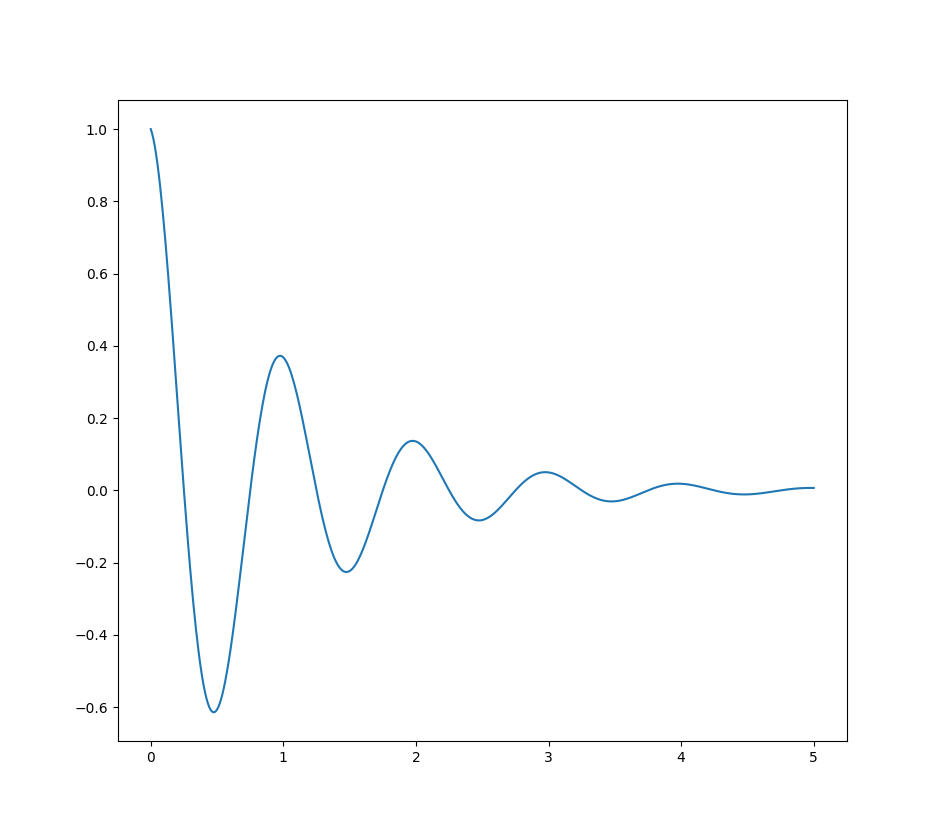
\includegraphics[width=0.49\linewidth]{TP07_exp.png}
\hfill
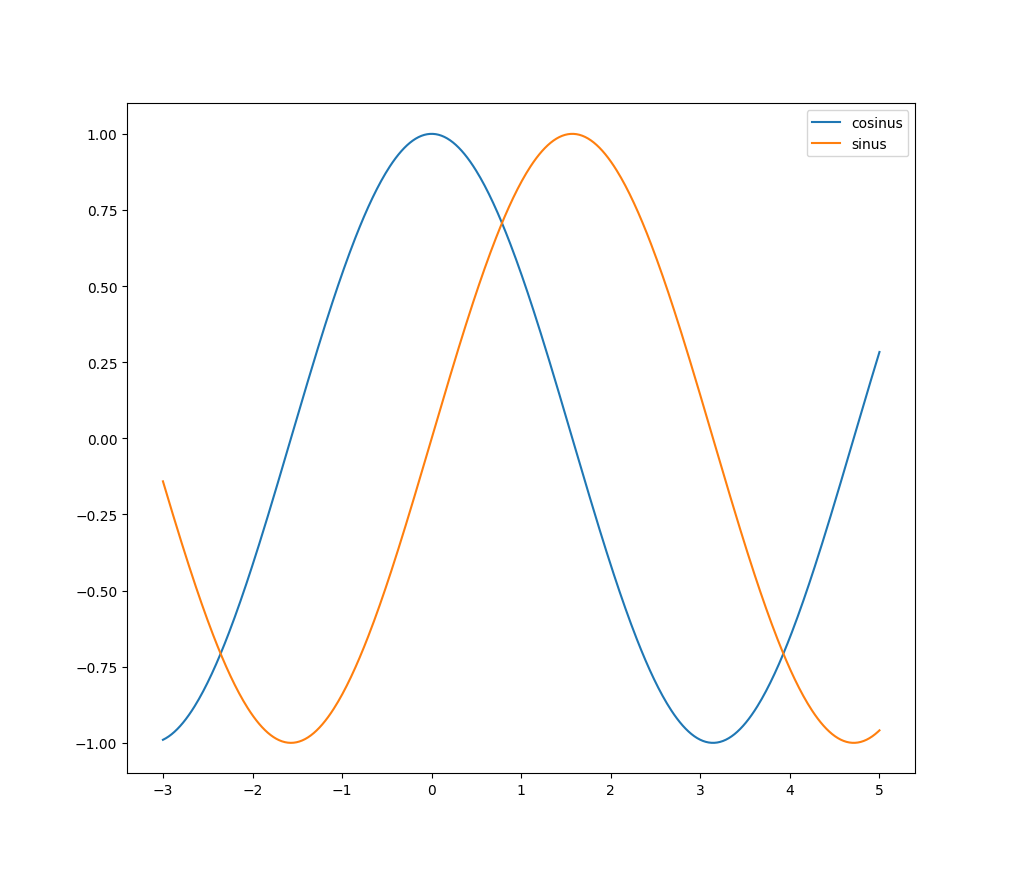
\includegraphics[width=0.49\linewidth]{TP07_cos_sin.png} 
\end{center}
%-------------------------------------------------------------------------------
%-------------------------------------------------------------------------------
%-------------------------------------------------------------------------------
\section{Tirages aléatoires  } 
%-------------------------------------------------------------------------------
%-------------------------------------------------------------------------------
%-------------------------------------------------------------------------------
Dans le module \type{random}, la fonction à deux variables entières \type{randint(a, b)} renvoie un entier au hasard compris entre $a$ et $b$ avec $a$ et $b$ compris.
%-------------------------------------------------------------------------------
\begin{lstlisting}
from random import randint
print(randint(4, 12))
\end{lstlisting}
%-------------------------------------------------------------------------------
On obtient un entier différent à chaque appel appartenant à $\{4, 5, \ldots, 12\}$.
%-------------------------------------------------------------------------------
%-------------------------------------------------------------------------------
\begin{Exercise}[title= Tirages de dés]\it
Écrire une fonction \type{tiragesDe(n)} qui renvoie une liste de taille $n$ dont les valeurs sont choisies aléatoirement entre 1 et 6.

Par exemple \type{tiragesDe(12)} peut renvoyer 
\type{[6, 5, 3, 3, 2, 2, 6, 4, 6, 5, 6, 1]}.
%-------------------------------------------------------------------------------
\end{Exercise}
%-------------------------------------------------------------------------------
\begin{Answer}
\begin{lstlisting}
from random import randint

def tiragesDe(n):
 	"""Entrée : un entier positif
 	   Sortie : la liste des tirages de n dés""" 
    resultat = [0]*n
    for i in range(n):
        resultat[i] = randint(1, 6)
    return resultat
\end{lstlisting}
\newpage
\end{Answer}
%-------------------------------------------------------------------------------
%-------------------------------------------------------------------------------
\begin{Exercise}[title= Occurrences]\it
Écrire une fonction \type{occurrences(liste)} qui renvoie une liste de taille 6 dont les valeurs sont les nombres d’occurrences des entiers de 1 à 6 dans une liste ne contenant que des entiers entre 1 et 6. Le terme d'indice $i$ de la liste ($0\le i < 6$) contiendra le nombre d’occurrences de $i+1$.
%-------------------------------------------------------------------------------
\end{Exercise}
%-------------------------------------------------------------------------------
\begin{Answer}
\begin{lstlisting}
def occurrences(liste):
 	"""Entrée : un entier positif
 	   Sortie : la liste de la distribution des valeurs
 	            d'une liste d'entiers de 1 à 6""" 
    n = len(liste)
    resultat = [0]*6
    for i in range(n):
        k = liste[i] - 1
        resultat[k] += 1
    return resultat
\end{lstlisting}
\end{Answer}
%-------------------------------------------------------------------------------
%-------------------------------------------------------------------------------

\medskip

\begin{minipage}[b]{0.55\textwidth}

On peut représenter le résultat par un histogramme.

\begin{enumerate}
\item On crée une liste de tirages : \type{T = tiragesDe(1200)}.
\item On répartit les tirages : \type{occ = occurrences(X)}.
\item On crée la liste des valeurs comptées : \type{X = [1, 2, 3, 4, 5, 6]}
\item On trace le graphe en barres
\begin{lstlisting}
plt.bar(X, occ)
plt.show()
\end{lstlisting}
\end{enumerate}
\end{minipage}
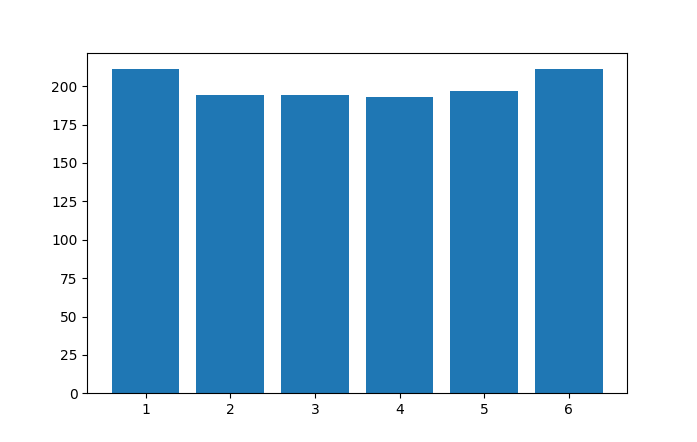
\includegraphics[width=0.50\linewidth]{TP07_des.png} 
%-------------------------------------------------------------------------------
%-------------------------------------------------------------------------------
%-------------------------------------------------------------------------------
\section{Suites} 
%-------------------------------------------------------------------------------
%-------------------------------------------------------------------------------
%-------------------------------------------------------------------------------
On a déjà vu la suite des nombres de Fibonacci ils sont définis par

\begin{center}
$F_0 = 0,\ F_1 = 1 \hbox{ et }F_{n+2} = F_{n+1} + F_n \hbox{ pour }n\in {\mathbb N}$
\end{center}
\vskip -5mm
%-------------------------------------------------------------------------------
%-------------------------------------------------------------------------------
\begin{Exercise}[title=Nombres de Fibonacci]\it
Écrire une fonction \type{liste\_fibo(n)} qui renvoie la liste formée des $n+1$ premiers nombres de Fibonacci, de $F_0$ à $F_n$. On notera qu'on doit renvoyer $n+1$ valeurs.
\end{Exercise}
%-------------------------------------------------------------------------------
\begin{Answer}
%-------------------------------------------------------------------------------
\begin{lstlisting}
def liste_fibo(n)
    F = [0]*(n+1)
    F[1] = 1 # F[0] vaut déjà 0
    for k in range(n-1): # 
        F[k+2] = F[k+1] + F[k] 
    return F
\end{lstlisting}
%-------------------------------------------------------------------------------
\end{Answer}
%-------------------------------------------------------------------------------
%-------------------------------------------------------------------------------

\medskip

Les nombres de Catalan sont des entiers qui apparaissent dans de nombreux problèmes de dénombrement.
Une de leurs définitions est la récurrence :

\begin{center}
$\displaystyle C_0 = 1 \hbox{ et }C_{n+1}=\sum_{i=0}^n C_iC_{n-i}\hbox{ pour }n\in {\mathbb N}$
\end{center}
\vskip -5mm
%-------------------------------------------------------------------------------
%-------------------------------------------------------------------------------
\begin{Exercise}[title=Nombres de Catalan]\it 
Écrire une fonction \type{catalan(n)} qui renvoie la liste formée des nombres de Catalan de $C_0$ à $C_n$.

\end{Exercise}
%-------------------------------------------------------------------------------
\begin{Answer}
\begin{lstlisting}
def catalan(n):
 	"""Entrée : un entier positif
 	   Sortie : la liste des nombres de catalan de C(0) à C(n)"""
    C = [0]*(n+1)
    C[0] = 1
    for k in range(n): # On calcule C(k+1)
        somme = 0
        for i in range(k+1): # i de 0 à k 
            somme = somme + C[i]*C[k-i] 
        C[k+1] = somme 
    return C
\end{lstlisting}
\end{Answer}
%-------------------------------------------------------------------------------
%-------------------------------------------------------------------------------
\medskip

On rappelle qu'on a $\displaystyle  \binom n{k+1} = \frac{n-k}{k+1} \binom nk$.
%-------------------------------------------------------------------------------
%-------------------------------------------------------------------------------
\begin{Exercise}[title= {Coefficients binomiaux, bis}]
Écrire une fonction \type{liste\_binom(n)} qui renvoie la liste des $\binom nk$ pour $0\le k \le n$.
\end{Exercise}
%-------------------------------------------------------------------------------
\begin{Answer} 
\begin{lstlisting}
def liste_binom(n):
    bin = [0]*n
    bin[0] = 1
    for k in range(n):
        bin[k+1 = bin[k]*(n-k)//(k+1)
    return bin
\end{lstlisting}
\end{Answer}
%-------------------------------------------------------------------------------
%-------------------------------------------------------------------------------
%-------------------------------------------------------------------------------
\section{Transformations de listes} 
%-------------------------------------------------------------------------------
%-------------------------------------------------------------------------------
%-------------------------------------------------------------------------------
\begin{Exercise}[title= Échanges]
Écrire une fonction \type{echanger(liste, i, j)} qui échange les termes d'indices $i$ et $j$ dans la liste. Cette fonction ne renvoie rien, elle doit modifier la liste.
\end{Exercise}
%-------------------------------------------------------------------------------
\begin{Answer} 
\begin{lstlisting}
def echanger(liste, i, j):
    temp = liste[i]
    liste[i] = liste[j]
    liste[j] = temp
\end{lstlisting}
\medskip
\end{Answer}
%-------------------------------------------------------------------------------
%-------------------------------------------------------------------------------

\medskip

Si on veut retourner une liste, on peut le faire en créant une nouvelle liste. Le plus simple alors est d'en extraire les termes "à l'envers" : \type{etsil = liste[ : : -1]}.

Dans ce qui suit on voudra effectuer les modifications en interne, 

on parle de transformation {\bf en place}. 

%-------------------------------------------------------------------------------
%-------------------------------------------------------------------------------
\begin{Exercise}[title= Retourner une liste]\it
%-------------------------------------------------------------------------------
Écrire une fonction \type{retourner(liste)} qui retourne une liste en place.
%-------------------------------------------------------------------------------
\end{Exercise}
%-------------------------------------------------------------------------------
\begin{Answer}
On utilise la fonction \type{echanger}.

On échange les termes symétriques en s'arrêtant à la moitié de la longueur, sinon on revient à la liste initiale. On doit échanger les éléments d'indice 0 à $p-1$ avec leur symétrique si $n=2p$ ou $n=2p+1$ (le milieu reste en place), on s'arrête à $\big\lfloor \frac n2 \bigr\rfloor - 1$.
%-------------------------------------------------------------------------------
\begin{lstlisting}
def retourner(liste):
    n = len(liste)
    for i in range(n//2): 
        echanger(liste, i, n-1-i)
\end{lstlisting}
\end{Answer}
%-------------------------------------------------------------------------------
%-------------------------------------------------------------------------------

\medskip

On se pose maintenant le problème de décaler une liste avec rotation vers la droite : les derniers éléments reviennent en tête.

Par exemple un décalage d'une place de \type{[4, 2, 8, 7, 5, 2, 1]} doit être \type{[1, 4, 2, 8, 7, 5, 2]}
%-------------------------------------------------------------------------------
%-------------------------------------------------------------------------------
\begin{Exercise}[title= Décaler d'une place]\it
%-------------------------------------------------------------------------------
Écrire une fonction \type{decaler1(liste)} qui décale une liste d'une position en place.
%-------------------------------------------------------------------------------
\end{Exercise}
%-------------------------------------------------------------------------------
\begin{Answer}
On place les éléments décalés depuis la fin. On doit conserver la valeur finale pour l'affecter à \type{liste[0]} à la fin.
\begin{lstlisting}
def decaler1(liste):
    n = len(liste)
    temp = liste[-1]
    for i in range(n-1, 0, -1): 
        liste[i] = liste[i-1]
    liste[0] = temp
\end{lstlisting}
\end{Answer}
%-------------------------------------------------------------------------------
%-------------------------------------------------------------------------------
\begin{Exercise}[title= Décalage]\it
%-------------------------------------------------------------------------------
En déduire une fonction \type{decaler(k, liste)} qui décale une liste de $k$ positions vers la droite.
%-------------------------------------------------------------------------------
\end{Exercise}
%-------------------------------------------------------------------------------
\begin{Answer}
\begin{lstlisting}
def decaler(k, liste):
    for i in range(k):
        decaler1(liste)
\end{lstlisting}
\end{Answer}
%-------------------------------------------------------------------------------
%-------------------------------------------------------------------------------
\medskip

Le décalage suggéré ci-dessus demande beaucoup d'affectations.

Il existe une astuce qui effectue moins de calculs. On va l'illustrer sur l'exemple ci-dessus.

\begin{enumerate}
\item Le décalage de 3 places de \type{[1, 4, 2, 8, 7, 5, 2]} est \type{[7, 5, 2, 1, 4, 2, 8]}.
On voit que les 3 derniers termes sont en tête et les $7-3$ premiers termes sont maintenant à la fin.
\item Si on retourne la liste on arrive à \type{[2, 5, 7, 8, 2, 4, 1]}, on voit que les 3 derniers termes sont maintenant en tête mais ils sont à l'envers, de même pour les $7-3$ premiers termes arrivés à la fin et retournés.
\item On retourne alors la portion des 3 premiers termes, on arrive à \type{[7, 5, 2, 8, 2, 4, 1]}.
\item On retourne les $7-3$ derniers termes, on aboutit à la liste décalée.
\end{enumerate}
%-------------------------------------------------------------------------------
%-------------------------------------------------------------------------------
\begin{Exercise}[title= Retournement partiel]\it
%-------------------------------------------------------------------------------
Écrire une fonction \type{inverser(liste, i, j)} qui retourne en place les éléments de la liste compris entre les position $i$ et $j$, borne $i$ comprise et borne $j$ exclue.
%-------------------------------------------------------------------------------
\end{Exercise}
%-------------------------------------------------------------------------------
\begin{Answer}
Si $j = i + 2p$, il y a un nombre pairs d'éléments à inverser : on échange $i$ et $j-1$, $i+1$ et $j-2$, jusqu'à $i + p-1$ et $i+p$.

Si $j = i + 2p+1$, il y a un nombre impairs d'éléments à inverser : on échange $i$ et $j-1$, $i+1$ et $j-2$, jusqu'à $i + p -1$ et $i+p+1$. L'élément d'indice $i+p$ est laissé à sa place. 

Dans les deux cas, la première coordonnée $k$ varie dans \type{range(i, i+p)} ; on a $\displaystyle i+p = \left\lfloor \frac{i+j}2 \right\rfloor$. La seconde coordonnée est $i+j-k-1$. 

\begin{lstlisting}
def inverser(liste, i, j):
    m = (j + i)//2
    for k in range(i, m):
        echanger(liste, k, i + j - k -1)
\end{lstlisting}
\end{Answer}
%-------------------------------------------------------------------------------
%-------------------------------------------------------------------------------
\begin{Exercise}[title= Décalage]\it
%-------------------------------------------------------------------------------
En déduire une fonction \type{decaler(k, liste)} qui décale une liste de $k$ positions vers la droite.
%-------------------------------------------------------------------------------
\end{Exercise}
%-------------------------------------------------------------------------------
\begin{Answer}
\begin{lstlisting}
def decaler(k, liste):
    n = len(liste)
    retourner(liste)
    inverser(liste, 0, k)
    inverser(liste, k, n)
\end{lstlisting}
\newpage
\end{Answer}
%-------------------------------------------------------------------------------
%-------------------------------------------------------------------------------
%-------------------------------------------------------------------------------
\section{En plus} 
%-------------------------------------------------------------------------------
%-------------------------------------------------------------------------------
%-------------------------------------------------------------------------------
\begin{Exercise}[title= Drapeau polonais]\it
%-------------------------------------------------------------------------------
Une liste ne contient que les valeurs 0 et 1. Écrire une fonction qui transforme la liste en plaçant tous 0 avant les 1 (on obtient 2 bandes, comme le drapeau polonais).
%-------------------------------------------------------------------------------
\end{Exercise}
%-------------------------------------------------------------------------------
\begin{Answer}

En plus de l'indice de boucle $i$, on utilise une variable $k\le i$ telle que :

les éléments d'indices entre 0 et $k-1$ sont 0

les éléments d'indices entre k et $i-1$ sont 1

\begin{lstlisting}
def zero_un(liste):
    n = len(liste)
    k = 0
    for i in range(n):
        if liste[i] == 0:
            echanger(liste, k, i)
            k = k + 1
\end{lstlisting}
\end{Answer}
%-------------------------------------------------------------------------------
%-------------------------------------------------------------------------------
\medskip

Si on remplace \type{liste[i] == 0} par \type{liste[i] < p} et \type{liste[i] == 1} par \type{liste[i] >= p}, on obtient un algorithme de séparation qui sera utile dans le tri rapide.
%-------------------------------------------------------------------------------
%-------------------------------------------------------------------------------
\begin{Exercise}[title= Drapeau hollandais]\it
%-------------------------------------------------------------------------------
Une liste ne contient que les valeurs $-1$, 0 et 1. Écrire une fonction qui transforme la liste en plaçant les termes dans l'ordre. On obtient 3 bandes, comme le drapeau néerlandais.Le concepteur de cet algorithme est  Edsger Dijkstra, qui est hollandais.
%-------------------------------------------------------------------------------
\end{Exercise}
%-------------------------------------------------------------------------------
\begin{Answer}
Ici utilise deux variables, $k_1$ et $k_2$.

les éléments d'indices entre 0 et $k_1-1$ sont -1

les éléments d'indices entre $k_1$ et $k_2-1$ sont 0

les éléments d'indices entre $k_2$ et $i-1$ sont 1

\begin{lstlisting}
def flag(liste):
    n = len(liste)
    k1 = 0
    k2 = 0
    for i in range(n):
        if liste[i] == -1:
            echanger(liste, i, k2)
            echanger(liste, k1, k2)
            k1 = k1 + 1
            k2 = k2 + 1
        if liste[i] == 0:
            echanger(liste, i, k2)
            k2 = k2 + 1
\end{lstlisting}
\end{Answer}
%-------------------------------------------------------------------------------
%-------------------------------------------------------------------------------
\medskip

Cet algorithme permet de séparer selon un pivot $p$ : les termes strictement inférieur à $p$, les termes égaux à $p$ et les termes strictement supérieur à $p$.












% \begin{Exercise}[title= Insertion dans une liste]
% %-------------------------------------------------------------------------------
% Écrire une fonction \type{inserer(x,i,liste)} qui renvoie une nouvelle liste où, à partir de \type{liste}, on a inséré l'élément \type{x} à la position \type{i} et décalé les suivants vers la droite.
% \end{Exercise}
% %-------------------------------------------------------------------------------
% \begin{Answer}
% le plus simple est d'utiliser les extractions.

% On rappelle que \type{liste[:i]+liste[i:]} reconstitue la liste.
% %-------------------------------------------------------------------------------
% \begin{lstlisting}
% def inserer(x,i,liste):
%     """Entrée : un élément x, un entier i et une liste
%                 on doit avoir 0 <= i <= len(liste)
%       Sortie : la liste avec x inséré à la position i"""
%     return liste[:i]+[x]+liste[i:]
% \end{lstlisting}
% \end{Answer}
% %-------------------------------------------------------------------------------
% %-------------------------------------------------------------------------------
% \begin{Exercise}[title= Suppression d'une position]
%  Écrire une fonction \type{supprimer\_place(i, liste)} qui renvoie une nouvelle liste où, à partir de \type{liste}, on a supprimé l'élément d'indice \type{i}. Les éléments suivants doivent être décalés vers la gauche.
% \end{Exercise}
% %-------------------------------------------------------------------------------
% \begin{Answer}
% \begin{lstlisting}
% def supprimer_place(i,liste):
%     """Entrée : un entier i et une liste, 0 <= i < len(liste)
%       Sortie : la liste moins le i-ième élément"""
%     return liste[:i]+liste[i+1:]
% \end{lstlisting}
% \end{Answer}
% %-------------------------------------------------------------------------------
% %-------------------------------------------------------------------------------
% \begin{Exercise}[title=Maximum]
% Écrire une fonction qui calcule le maximum des termes d'une liste.
% \end{Exercise}
% %-------------------------------------------------------------------------------
% \begin{Answer}
% %-------------------------------------------------------------------------------
% \begin{lstlisting}
% def maxListe(liste):
% 	  """Entrée : une liste non vide
% 	     Sortie : la valeur du maximum de la liste"""
%   maximum = liste[0] # Un maximum provisoire
%   n = len(liste)
%   for i in range(n):
%       if maximum < liste[i]:
%           maximum = liste[i]
%   return maximum
% \end{lstlisting}
% %-------------------------------------------------------------------------------
% On compare inutilement le premier terme avec lui-même pour $i=0$. On pouvait écrire \type{for i in range(1,n)}, dans le cas $n=1$ aucune itération n'est calculée.

% \medskip

% On pouvait aussi se passer de l'indice :
% %-------------------------------------------------------------------------------
% \begin{lstlisting}
% def maxListe(liste):
%  	"""Entrée : une liste non vide
% 	     Sortie : la valeur du maximum de la liste"""
%   maximum = liste[0] # Un maximum provisoire
%   for x in liste:
%       if maximum < x:
%           maximum = x
%   return maximum
% \end{lstlisting}
% %-------------------------------------------------------------------------------
% \end{Answer}


% %-------------------------------------------------------------------------------
% %-------------------------------------------------------------------------------
% \begin{Exercise}[title=Transformation de Cesàro]

% La transformée de Cesàro\footnote{D'après le lemme de Cesàro, si une suite converge vers $\ell$,  sa transformée de Cesàro converge vers $\ell$ aussi.} d'une suite $(u_n)$ est la suite $(v_n)$ définie par $\displaystyle v_n= \frac 1{n +1}\sum_{k=0}^n u_k$. 



%  Écrire une fonction \type{cesaro(liste)} qui renvoie les $n$ premiers termes de la transformée de Cesàro d'une suite donnée par les éléments de la liste de longueur $n$.
% %-------------------------------------------------------------------------------
% \end{Exercise}
% %-------------------------------------------------------------------------------
% \begin{Answer}
% \begin{lstlisting}
% def cesaro(liste):
%     """Entrée : une liste de nombre
%       Sortie : la suite transformée de Cesaro"""
%     n = len(liste)
%     ces = [0]*n
%     somme = 0
%     for k in range(n):
%         somme = somme + liste[k]
%         ces[k] = somme/(k+1)
%     return ces
% \end{lstlisting}
% %-------------------------------------------------------------------------------
% \end{Answer}
% %-------------------------------------------------------------------------------
% %-------------------------------------------------------------------------------


